\chapter{Introduction}
\section{The synthesis imaging widefield problem}
In radio astronomy there is a well-known Fourier relationship between the sky brightness distribution and the measurements taken by antenna arrays, see for instance 
Clark \cite[Lecture 1]{taylor1999synthesis}. To synthesize an image of the sky intensity distribution the measurements taken by these so-called radio \textit{interferometers}
are normally inverted by resampling the points onto a regularly-spaced grid and performing an inverse Fast Fourier Transform \cite{cochran1967fast} on the resampled measurements, see for instance 
Thompson \cite{thompson1974interpolation}. The synthesized images are convolved with the inverse of the sampling pattern of the array, requiring that
the inversion step be called upon multiple times in an iterative deconvolution strategy such as Cotton-Schwab CLEAN (see Thompson et al. \cite[ch 11]{thompson2008interferometry}).

When synthesizing wide field images using an array of telescopes with non-East-West antenna pair ``baselines'' the simple Fourier relationship between the sky brightness 
distribution and interferometer measurements break down, because of a combination of two factors: the Fast Fourier Transform only approximates the sky by a plane, and secondly 
the measurements taken by the telescope do not remain coplanar over the course of longer observations. Due to this ``tilting'' of the sampling plane the projected position of 
sources far away from the centre of the synthesized fields do not remain constant and the brightness of the sources is smeared out over time. These two sources of error is 
collectively known as the problem of \textit{non-coplanar widefield imaging}, see for instance Cornwell and Perley \cite{cornwell1992radio}.

One strategy for resolving the sources affected by this smearing is to split the sky up into small narrow field (``facet'') images, tiling the sky in a 
polyhedron-like fashion \cite{cornwell1992radio}. The synthesized images produced by such a non-coplanar faceting approach is hard to deconvolve and 
require reprojection and intensity correction in the overlapping areas. Another strategy uses 
convolution to introduce a correcting phase shift into each of the individual measurements taken by the instrument over time and is known as w-projection \cite{cornwell2008noncoplanar}. This approach
relates the non-coplanar measurements to a single plane, eliminating the phase delay introduced by the tilted interferometer baselines. 

In w-projection the resampling cost can be related to the size of the produced images, where as in traditional faceting the cost rise with number of facets. Unlike w-projection faceting 
is less memory intensive, especially for large images and arrays with very long baseline components. The work in this thesis concentrates on creating coplanar facet images by combining facet 
imaging and w-projection in what we call \textit{w-faceting}. Due to the nature of imaging using interferometers it is desirable to have baselines as long as possible to improve the resolving
capability of the telescope, enough baselines in-between to create uniform sampling coverage in the measurement domain and as much collecting area as possible to improve the sensitivity of 
the instrument. Instruments such as the Square Kilometre Array \cite{carilli2004science} and its pathfinders MeerKAT \cite{booth2009meerkat} and ASKAP \cite{johnston2008science} have significantly more
baselines than some of their predecessors, such as the Jansky Very Large Array \cite{2041-8205-739-1-L1}. As the baselines grow roughly as the square of the number of antennas, and improved spatial resolving 
capability and sensitivity decreases the integration time for each measurement made per baseline the data rates from these telescopes provide a tough computational problem for image synthesis. Luckily due to
the linearity of the underlying relationship between the sky and the measurements, and the dimensions of the input data and output products, the synthesis pipeline lends itself to the parallel and 
distributed nature of modern processing equipment. The work in this thesis focus on investigating resampling scalability within shared memory environments, comparing CPU- and GPU-based w-facet imaging.
Distributed implementation is not within the scope of this work, although the shared memory w-facet technique can be expanded to include multiple processing cluster nodes due to its data-parallel 
nature.
\section{Research questions and aims}
We have identified the following research questions for our research:
\begin{enumerate}
 \item Is GPU-based w-faceting more scalable than a CPU-based parallel and vectorized implementation?
 \item Does single precision gridding introduce any significant error in the synthesized images?
 \item What effect does double precision resampling have on resampling performance?
\end{enumerate}

The aim of this work is to build a scalable w-facet imager. At present a full accelerated deconvolution pipeline implementation is out of scope, and we will focus solely on the ``backward'' synthesis step
that includes the computationally expensive convolutional resampling step necessary to take the Inverse Fast Fourier Transform. Our imager will also support the ability to target regions of the sky in what is
appropriately called \textit{targeted faceting}.

\section{Software approach}
To enable our investigation into scalability we have build our own targeted facet imaging framework called \textit{Bullseye}. The software package and source code is publicly available at the Rhodes University Radio Astronomy 
Techniques and Technologies Group repository \url{https://www.github.com/ratt-ru/bullseye} under the GNU General Public License. Our framework includes a command-line utility with options similar to those provided by other imagers such 
as WSClean \cite{offringa2014wsclean} and CASA \cite{jaeger2008common,mcmullin2007casa}. The package reads radio measurement information from the widely-used Measurement Set \cite{ms10,ms20} format standard and writes the synthesized 
orthogonally-projected dirty facet images out in the widely employed Flexible Image Transport System \cite{pence2010definition,calabretta2002representations} standard. Figure~\ref{fig_aims_pipeline} shows the focus of our work
within the synthesis imaging pipeline.
\begin{figure}
 \begin{mdframed}
  \centering
  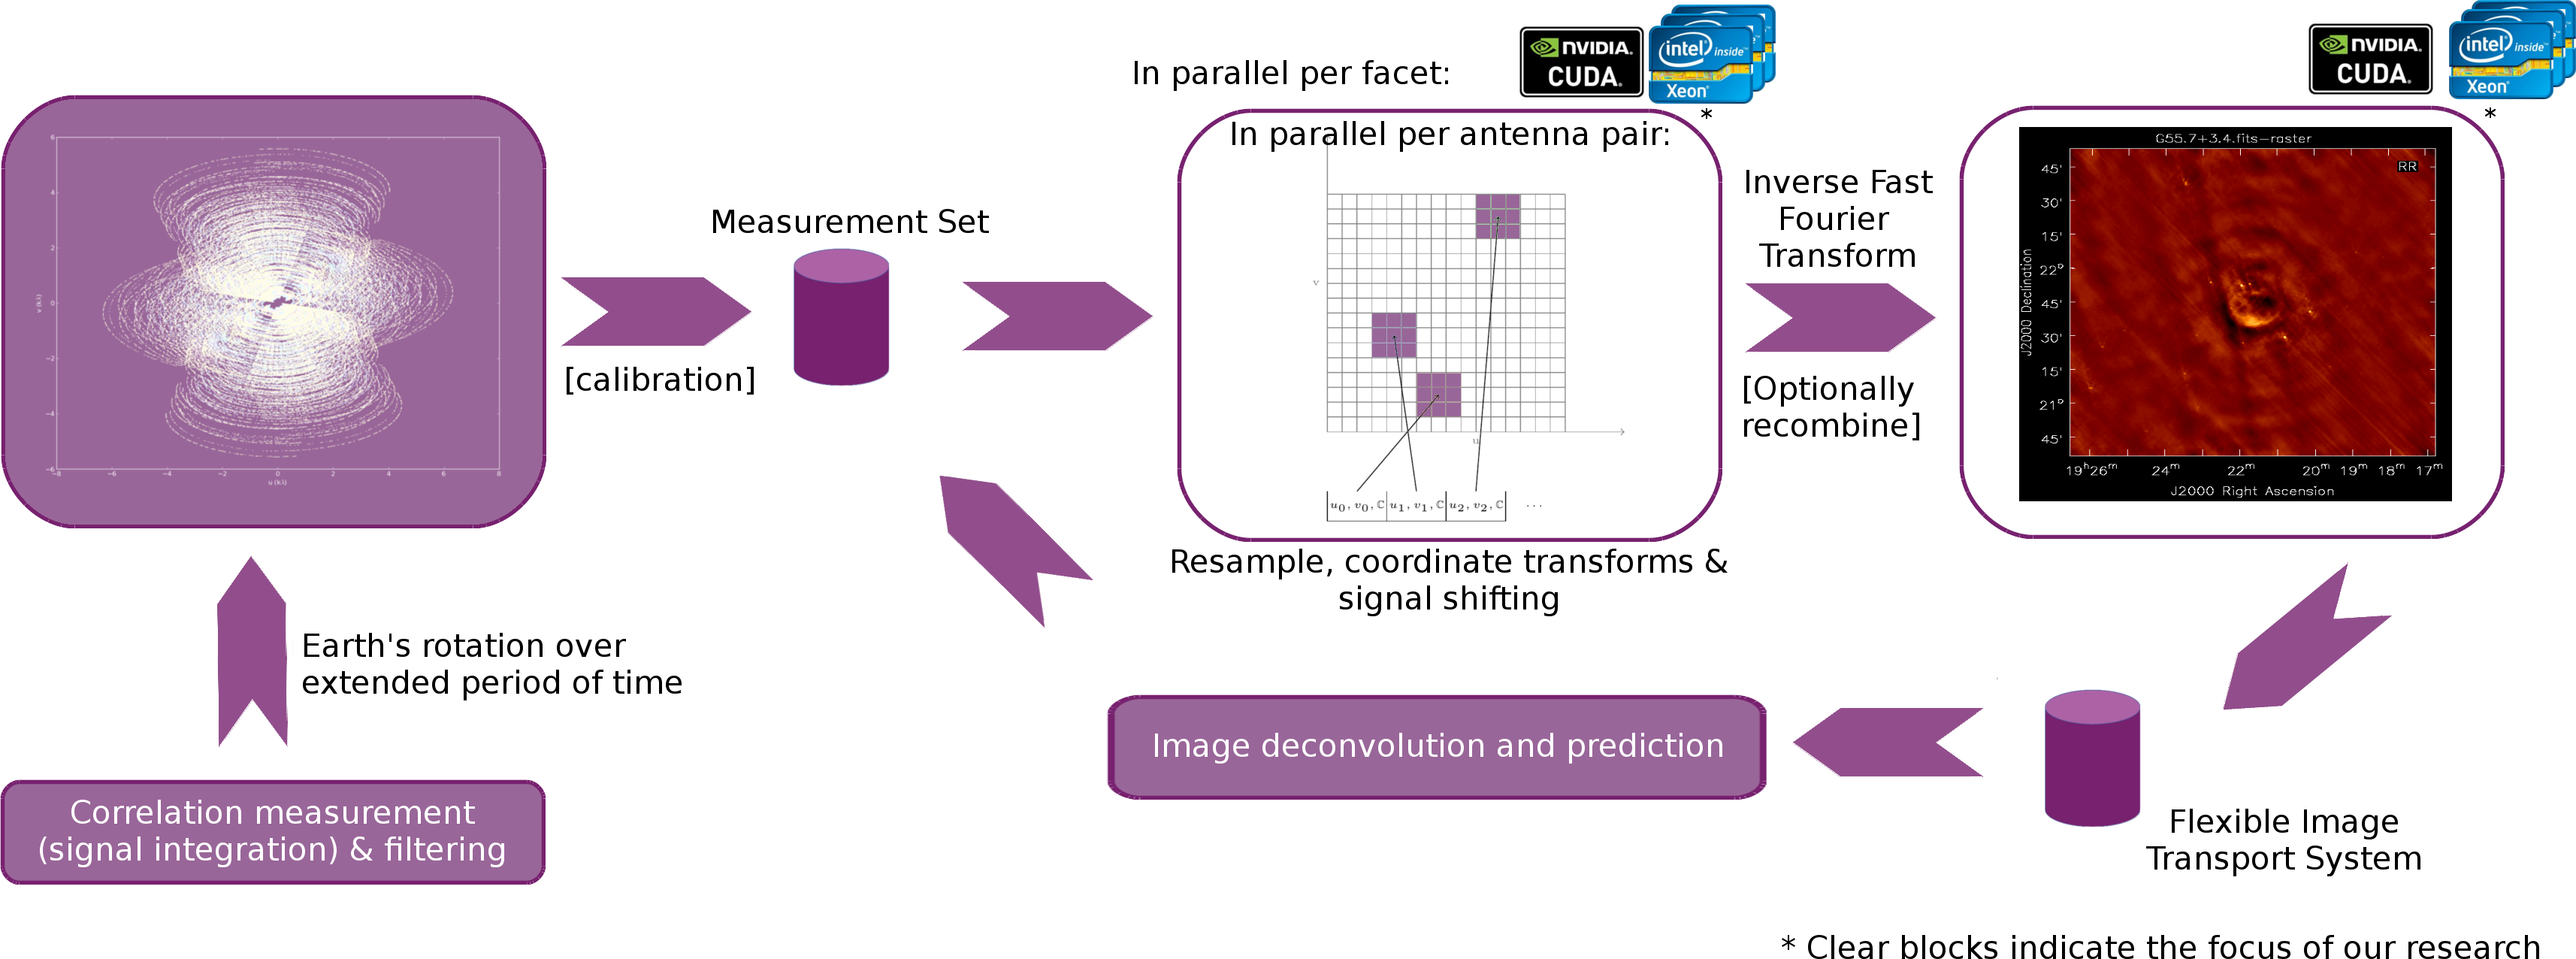
\includegraphics[width=0.95\textwidth]{images/aims_process.png}
  \caption[Aims of the work in this thesis and position in synthesis pipeline.]{This pipeline illustrates the major steps in the synthesis imaging and deconvolution pipeline. Our work focus on parallelizing the resampling,
	  coordinate and data transform steps that are necessary to take the Inverse Fast Fourier Transform to synthesize dirty facets. Both the major and minor cycle deconvolution and associated prediction step is out of scope for our work.}
  \label{fig_aims_pipeline}
 \end{mdframed}
\end{figure}

\section{Outline}
The discussion in this document is divided into the following sections:
\begin{itemize}
 \item \textbf{Chapter 2: Review of multi- and many-core processing models} gives readers not familiar with recent trends in CPU and GPU design an architectural overview of each, and a discussion
 on the processing terminology used in later chapters. 
 \item \textbf{Chapter 3: The Radio Interferometric Measurement Equation} is aimed at readers coming from an engineering background or those unfamiliar with radio interferometry. The chapter 
 gives a basic overview of radio interferometry, associated coordinate systems and derives the formal mathematical model for the relationship between the sky and the measurement domain.
 \item \textbf{Chapter 4: Wide field image synthesis} discusses the inversion process of the Radio Interferometric Measurement Equation and the associated wide field problems 
 in more technical detail than that given in the overview above. This technical discussion leads on directly to the imager design chapter.
 \item \textbf{Chapter 5: Bullseye: A parallel targeted facet imager} discusses the architectural design, processing algorithms used in our imager and our validation strategy.
 \item \textbf{Chapter 6: Performance analysis} discusses imager performance in terms scalability and accuracy.
 \item \textbf{Chapter 7: Conclusion and future work} highlights the key findings made in the analysis and outlines the key areas where future work and investigation is necessary.
\end{itemize}
